\chapter{Konzeption Publish/Subscribe-Systeme}
\label{chap:konzeption_pubsub}
Diese Arbeit entwickelt ein Framework auf Basis eines strukturierten P2P-Overlay-Netzwerkes. Die im System nutzbaren Publish/Subscribe-Systeme müssen ebenfalls verteilt arbeiten können. Dabei spielen die Fehlertoleranz und auch die Fähigkeit mit \emph{churn}, d.h. schnellem Wechsel der Mitgliedschaften, umgehen zu können.

Zur Konzeption des Frameworks werden anhand dreier prominenter Systeme Gemeinsamkeiten identifiziert und generalisiert. Diese drei Systeme sind \begin{inparaenum}[(1]) \item Scribe \cite{Castro2002Scribe}, \item VON \cite{Hu2006VON} und \item MercuryMercury \end{inparaenum}. Scribe und VON sind kanalbasierte Publish/Subscribe-Systeme, Mercury hingegen ist filterbasiert. Obwohl das Framework im jetzigen Entwicklungsstand auf kanalbasierte Systeme beschränkt ist \missing{Erklärung warum}, kann der Algorithmuns hinter Mercury interessante Einblicke und Ideen liefern.


\section*{Scribe}
\label{chap:related:scribe}
Scribe \cite{Castro2002Scribe} gehört zur Klasse der kanalbasierten\footnote{siehe \Fref{chap:grundlagen:pubsub:kanalbasiert}} Publish/Subscribe-Systeme und basiert auf dem strukturierten Overlay-Netzwerk Pastry \cite{Rowstron2001}. Bayeux \cite{Zhuang2001} ist ein ähnliches System, jedoch auf Basis des Overlay-Netzwerkes Tapestry. Da beide dieser Netwerke der generischen API entsprechen, stellt dies keinen Unterschied dar.

Dabei nutzt Scribe einen vom Subscriber zum Publischer aufgebauten Baum \emph{reverse path forwarding tree} \cite{Dalal1978}. Im Gegensatz dazu nutzt Bayeux einen Baum der vom Publisher zum Subscriber augebaut wird. Aufgrund der unterliegenden Routingstruktur des genutzten Overlay-Netzwerkes können sich diese Pfade unterscheiden.

Der Vorteil von strukturierten Netzwerken ist, dass über einen berechneten Schlüssel der zuständige Knoten gefunden wird. Bei Scribe berechnet ein Knoten den Root-Knoten des Kanals über den Hashwert des Kanalnamens. Ein Subscriber lässt nun eine \emph{subscribe}-Nachricht an den entsprechenden Knoten routen. Alle Zwischenknoten empfangen diese Nachricht in \emph{forward}, tragen den Sender in eine Liste ein und subscriben sich selbst an diesem Kanal. Die ursprüngliche Nachricht wird terminiert. Wird eine weitere solche Nachricht empfangen, so muss lediglich der Absender in die Liste eingetragen werden. Weitere Nachrichten sind nicht erforderlich.\\
Ein Knoten, der eine Nachricht publizieren möchte, lässt das Netzwerk ebenfalle eine Nachricht an den Root-Knoten des Systems routen. Dieser Root-Knoten sendet die Nachricht an alle Knoten in der Liste. Diese Knoten verfahren ebenso und damit wandert die Nachricht den Baum hinab. Sind diese Knoten ebenfalls Subscriber wird die Nachricht an die Applikation weitergegeben.

\begin{figure}[htbp]
\centering
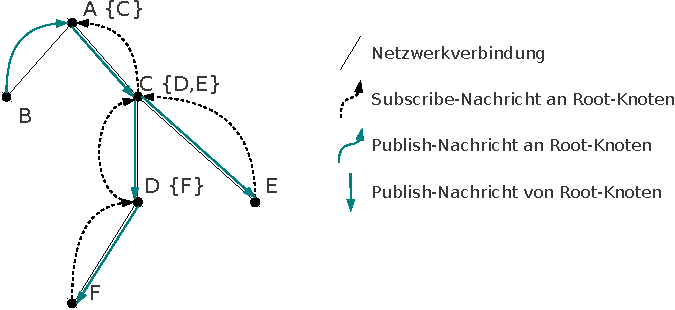
\includegraphics{grafics/multicast_tree.pdf}
\caption{Schema eines Multicast-Trees}
\label{fig:multicast_tree}
\end{figure}

\Fref{fig:multicast_tree} zeigt ein Netzwerk mit den sechs Knoten A-F. Die Verbindungen der Knoten werden durch dünne schwarze Linien dargestellt. Knoten C hat Verbindungen zu A, B, D und F. Knoten A ist der Root-Knoten des im Beispiel verwendeten Kanals, da er für den aus dem Hashwert des Kanalnamens berechneten Schlüssel zuständig ist.

\paragraph*{Subscribe} Knoten F sendet eine \emph{subscribe}-Nachricht an A. Knoten D muss diese Nachricht weiterleiten, lässt diese aber terminiern und trägt F in die Liste ein. Knoten D sendet nun selbst eine \emph{subscribe}-Nachricht an A. Diese Nachrichten sind in der Grafik durch gebogene schwarze Verbindungslinien mit Pfeil dargestellt. Nachdem sich auch Knoten E für den Kanal eingeschrieben hat, wurden im Netzwerk insgesamt vier Nachrichten versandt: F an D, D an C, C an A und E an C. Wenn die \emph{subscribe}-Nachricht von E C erreicht, wird E lediglich in die Liste eingetragen. Ein erneutes Anmelden von C entfällt.

\paragraph*{Publish} In \Fref{fig:multicast_tree} möchte Knoten B eine Nachricht im Kanal publizieren. B sendet darauf eine Nachricht an den Root-Knoten A, da dieser für diesen Kanal zuständig ist (gebogene türkise Linie). Nun sendet A diese Nachricht an alle Knoten in der Liste (gerader türkiser Pfeil). Knoten C sendet die Publikation von B an die Knoten D und E. E gibt diese Nachricht direkt an die Applikation weiter, während D die Nachricht an F schicken muss.

Hierbei ist klar ersichtlich, dass ein Overhead an Nachrichten entsteht, wenn Knoten F eine Nachricht im Kanal publizieren möchte. Diese Nachricht muss erst von Knoten F zu Knoten A wandern, nur damit A diese Nachricht wieder über die anderen Knoten zurücksendet. Optimierte Versionen dieses Algorithmus können hier ansetzen und zu publizierende Nachrichten nicht mehr an den Knoten senden, der ihnen diese Nachricht geschickt hat. So würde C die Nachricht gleich an E weiterleiten.


Obwohl dieses System die Anzahl der zu versendenden Nachrichten drastisch reduziert, ist anzumerken, dass Knotenpunkte Kanalnachrichten bearbeiten müssen, für die sie sich nicht interessieren. Beispielsweise ist Knoten A in \emph{TEAM RED}, ist aber berechneter Root-Knoten des Kanals \emph{TEAMSPEAK.TEAM\_EAGLE}.

Scribe fordert periodische Subscriptions zur Erhöhung der Fehlertoleranz.

\section*{VON}
\label{chap:related:von}
\cite{Hu2006VON} %VON

\cite{Backhaus2007Voronoibased} %VAST
\ac{vast}


\section*{Mercury}
\label{chap:related:mercury}
Mercury \cite{Bharambe2004Mercury} gehört zur Klasse der filterbasierten\footnote{siehe \Fref{chap:grundlagen:pubsub:filterbased}} Publish/Subscribe-Systeme \index{Publish/Subscribe!filterbasiert}.

\paragraph{Arbeitsweise}
Im System gibt es eine Menge an Attributen, die ihrerseits einen definierten Wertebereich haben. Jedes Attribut wird durch einen eigenen \emph{Hub}, ein Verbund aus Knoten, gebildet. Der Wertebereich ist dabei nicht zwingend symetrisch\footnote{Angenommen, $0<=x<360$: Knoten $A_{[0,270)}$, $B_{[270, 360)}$} auf die Knoten verteilt. Die Knoten eines Hubs sind sich untereinander über Nachbarschaftsmetriken\footnote{Alte Version: forward- und backward-Pointer; Ringstruktur\\Neue Version: Tabelle mit allen Knoten im Hub} bekannt.
Eine Subscription $S$ ist ein Tupel aus Filterbedingungen über die Attribute, bsp. $S := (5 < x <= 20; y = 15)$. $S$ wird nun an einen beliebigen Knoten eines Hubs gesendet, der für ein Attribut aus den Filterbedingungen zuständig ist. Im Hub wird $S$ nun zu dem Knoten weitergereicht, der den Wertebereich der Filterung abdeckt. Dort wird $S$ in einer Liste gespeichert.
Eine Publikation $P$ ist ebenfalls ein Tupel mit bestimmten Werten der Attribute, bsp. $P := (x = 10; y = 0)$. $P$ wird an \emph{alle} Hubs gesendet, die für Attribute aus dem Tupel zuständig sind. Dort wird $P$ zum zustädnigen Knoten weitergereicht. Dieser prüft nun die Liste der gespeicherten Subscriptions gegen die neue Publikation. Stimmen beide überein, so wird $P$ an den eingeschriebenen Knoten weitergeleitet.


\cite{BeFiMu2006PubSubQoS}

\cite{PiEyKoSh2007-PubSubAPI}

\cite{KostasKatrinis2005}
